\subsection{Laurent Series}
The Laurent series generalizes the Taylor series to holomorphic functions with isolated singularities. While Taylor series are valid within a disk centered at a point of holomorphy, Laurent series apply to annular regions surrounding a singularity, making them essential for studying functions near non-removable singularities (refer to \cref{thm:riemannremovablesingularities}).

We now introduce a fundamental result in complex analysis due to Weierstrass, which formalizes the conditions under which the limit of a sequence of holomorphic functions is itself holomorphic. This theorem not only guarantees the holomorphy of the limit function but also the uniform convergence of its derivatives (its statement was used in the proof of \cref{thm:hurwitzsimplecase}).
\begin{theorem}[Weierstrass]\label{thm:weierstrassconvergence}
    Let \(\cbraces{f_n(z)}_{n\in\mathbb{N}}\) be a sequence of holomorphic functions on an open region \(U\subseteq\mathbb{C}\) that converges uniformly to \(f(z)\) on every compact subset of \(U\). Then \(f(z)\) is holomorphic on \(U\), and \(\forall k\in\mathbb{N}\), the sequence \(\cbraces{f^{(k)}_n(z)}_{n\in\mathbb{N}}\) uniformly converges to \(f^{(k)}(z)\) on all compact subsets of \(U\).
\end{theorem}
\begin{proof}
    By Morera's Theorem (\cref{thm:morera}) and the uniform convergence of \(\cbraces{f_n(z)}\), the holomorphy of \(f(z)\) follows (refer to \cref{eq:hurwitzsimplecase_integrallimitswitchforholomorphy} and preceding explanations).

    Following the same logic, by \cref{cor:nthderivativeboundedsupremum}, \(\forall k\in\mathbb{N}\) and for all compact \(K\subset U\) and open \(V\supset K\) relatively compact in \(U\) there exists a finite constant \(c_k>0\) such that
    \[\lim_{n\to\infty}\sup_{z\in K}\abs{f_n^{(k)}(z)-f^{(k)}(z)}\leq c_k\lim_{n\to\infty}\sup_{z\in V}\abs{f_n(z)-f(z)}.\] Since \(\cbraces{f_n(z)}\) is uniformly convergent, the limit on the right-hand side vanishes. Then,
    \[\lim_{n\to\infty}\sup_{z\in K}\abs{f_n^{(k)}(z)-f^{(k)}(z)}=0,\] and therefore \(\cbraces{f^{(k)}_n(z)}\) uniformly converges on all compact subsets of \(U\).
\end{proof}
The condition of uniform convergence on every compact subset can also be significantly loosened, by the fact demonstrated below:
\begin{proposition}
    Let \(U\subseteq\mathbb{C}\) be an open bounded region, and let \(\cbraces{f_n(z)}\) be holomorphic on \(U\). Let \(K\subset U\) be compact. If \(f_n\rightrightarrows f\) on \(\partial K\), then \(f_n\rightrightarrows f\) on \(K\).
\end{proposition}
\begin{proof}
    By the converse statement of the Cauchy Criterion (\cref{thm:cauchycriterionuniformconvergence}), \(\forall\varepsilon>0\), \(\exists N\in\mathbb{N}\) such that \(\forall n,m>N\), \[\sup_{z\in\partial K}\qty|f_n(z)-f_m(z)|<\varepsilon.\]
    By the Maximum Modulus Principle (\cref{thm:maximummodulus}) on \(f_n-f_m\), \[\sup_{z\in\partial K}\abs{f_n(z)-f_m(z)}=\sup_{z\in K}\abs{f_n(z)-f_m(z)}<\varepsilon.\]
    It follows that \(f_n\rightrightarrows f\) on \(K\) by \cref{thm:cauchycriterionuniformconvergence}.
\end{proof}
\begin{remark}
    From the above result, the uniform convergence on every compact subset in \cref{thm:weierstrassconvergence} can therefore be loosened to the uniform convergence on every simple closed curve.
\end{remark}
We will now study Laurent series. Let \(a\in\mathbb{C}\) and \(\cbraces{c_n}_{n\in\mathbb{Z}}\subset\mathbb{C}\) be constants. A series in the form of
\begin{equation}\label{eq:laurentseries}
    f(z)=\sum_{n=-\infty}^\infty c_n(z-a)^n
\end{equation}
is a Laurent series at the point \(a\). The series can be separated into a power series with non-negative exponents,
\begin{equation}
    \varphi(z)=\sum_{n=0}^\infty c_n(z-a)^n,\label{eq:laurentseriesnonnegativeexponents}
\end{equation} and a power series with negative exponents,
\begin{equation}
    \psi(z)=\sum_{n=1}^{\infty}c_{-n}(z-a)^{-n}.\label{eq:laurentseriesnegativeexponents}
\end{equation} \cref{eq:laurentseries} is said to be convergent at \(z=z_0\) if the two power series are both convergent. Let the convergence radius of \cref{eq:laurentseriesnonnegativeexponents} be \(R=\frac{1}{\varlimsup_{n\to\infty}\sqrt[n]{\abs{c_n}}}\) by the Cauchy--Hadamard Theorem (\cref{thm:cauchyhadamard}). It follows that the \(\varphi\) is holomorphic on \(D(a,R)\). Let \(\zeta=(z-a)^{-1}\). Then \cref{eq:laurentseriesnegativeexponents} becomes \(\sum_{n=1}^\infty c_{-n}\zeta^n\). This series converges when \(\abs{\zeta}<\frac{1}{\varlimsup_{n\to\infty}\sqrt[n]{\abs{c_{-n}}}}=\lambda\). Let \(r=\frac{1}{\lambda}\). Then \(\psi(z)\) converges when \(\abs{z-a}>\varlimsup_{n\to\infty}\sqrt[n]{\abs{c_{-n}}}\), or when \(z\in\mathbb{C}\setminus\overline{D(a,r)}\).

If \(R>r\), then \(f\) is convergent on the annulus \(D(a,R)\setminus\overline{D(a,r)}\) and divergent on \(\mathbb{C}\setminus\overline{D(a,R)}\cup D(a,r)\). If \(r=R\), the series diverges possibly everywhere but on \(\partial D(a,r)\). Similar to power series with positive exponents, the convergence on the boundary varies. For example, \(\sum_{\substack{n=-\infty\\n\neq0}}^\infty\frac{z^n}{n^2}\), where \(R=r=1\), converges (absolutely) on \(\partial\mathbb{D}\), whereas \(\sum_{n=-\infty}^\infty z^n\) diverges on all of \(\partial\mathbb{D}\), while \(\sum_{\substack{n=-\infty\\n\neq0}}^\infty\frac{z^n}{n}\) converges (conditionally) on all of \(\partial\mathbb{D}\setminus\cbraces{1}\) and diverges at \(z=1\). If \(r>R\), then the series is divergent on all of \(\mathbb{C}\). The region \(D(a,R)\setminus\overline{D(a,r)}\) is known as the \textscsl{annulus of convergence}.\ \(f(z)\) in \cref{eq:laurentseries} is holomorphic over this annulus. The series \(\varphi(z)\) is known as the \textscsl{holomorphic part} of \(f(z)\), and \(\psi(z)\) is known as the \textscsl{principal part} of the Laurent series. The properties of the convergence disk in Abel's Theorem (\cref{thm:abelradius}) can be generalized to Laurent series. In other words, \(f\) is absolutely convergent on the annulus and is uniformly convergent on every compact subset of it.
\begin{theorem}\label{thm:laurentexpansionofholomorphicfunction}
    Let \(V=\cbraces{z\in\mathbb{C}}{r<\abs{z-a}<R}\) for some \(0\leq r<R\leq+\infty\). Let \(f\) be holomorphic on \(V\). Then \(f\) has the unique \textscsl{Laurent expansion}
    \begin{equation}
        f(z)=\sum_{n=-\infty}^\infty c_n(z-a)^n,\qquad c_n=\frac{1}{2\piup\ii}\oint_{\gamma}\frac{f(\zeta)\ddzeta}{(\zeta-a)^{n+1}},\qquad z\in V,\label{eq:laurentexpansionofholomorphicfunction_statement}
    \end{equation} for any simple closed curve \(\gamma\subset V\) enclosing \(a\). Moreover, the series converges absolutely on \(V\) and uniformly on all compact subsets of \(V\).
\end{theorem}
\begin{proof}
    \begin{figure}
        \centering
        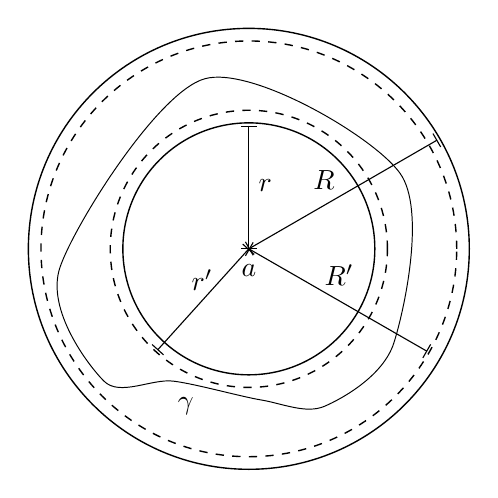
\begin{tikzpicture}\draw[line width=0.35] plot[smooth cycle] coordinates {
                    (-2.4,-0.24) (-1.84,-1.68) (-0.96,-1.68) (0.16,-1.92) (0.96,-2.0) (1.84,-1.2) (1.92,0.96) (-0.56,2.16)
                };
            \draw[line width=0.5] (2.8,0) arc[start angle=0, end angle=360, radius=2.8];
            \draw[line width=0.5, dashed] (2.64,0) arc[start angle=0, end angle=360, radius=2.64];
            \draw[line width=0.5] (1.6,0) arc[start angle=0, end angle=360, radius=1.6];
            \draw[line width=0.5, dashed] (1.76,0) arc[start angle=0, end angle=360, radius=1.76];
            \draw[thin, |-|, line cap=round, shorten >=1pt] (0,0) -- (2.424,1.4) node[midway, anchor=south east, yshift=-2pt] {\(R\)};
            \draw[thin, |-|, line cap=round, shorten >=1pt] (0,0) -- (0,1.6) node[midway, right] {\(r\)};
            \draw[thin, |-|, line cap=round, shorten >=1pt] (0,0) -- (2.296,-1.32) node[midway, anchor=south, yshift=2pt] {\(R'\)};
            \draw[thin, |-|, line cap=round, shorten >=1pt] (0,0) -- (-1.184,-1.312) node[midway, anchor=south] {\(r'\)};

            \node[anchor=north] at (0,-0.08) {\(a\)};
            \node[anchor=north] at (-0.8,-1.76) {\(\gamma\)};
        \end{tikzpicture}
        \caption{The annulus \(V\), with \(\gamma_1\), \(\gamma_2\), and \(\gamma\).}\label{fig:laurentexpansionofholomorphicfunction}
    \end{figure}By the openness of \(V\), there exist two circles \(\gamma_1\subset V\) with radius \(r'\) and \(\gamma_2\subset V\) with radius \(R'\) centered at \(a\) such that \(\gamma\) encloses \(\gamma_1\) and \(\gamma_2\) encloses \(\gamma\) both without intersection. Let \(W=\cbraces{z\in V}{r'<|z-a|<R'}\) and \(z\in W\) be arbitrary. By the Cauchy--Goursat Formula (\cref{thm:cauchygoursatformula}), \[f(z)=\frac{1}{2\piup\ii}\qty(\oint_{\gamma_2}\frac{f(\zeta)\ddzeta}{\zeta-z}-\oint_{\gamma_1}\frac{f(\zeta)\ddzeta}{\zeta-z}).\]
    \(\forall\zeta\in\gamma_1\) (or \(|\zeta-a|=r'\)), \(\abs{\zeta-a}<\abs{z-a}\) and therefore, \(\frac{\abs{\zeta-a}}{\abs{z-a}}<1\). It follows that
    \begin{equation}
        \frac{1}{\zeta-z}=-\frac{1}{(z-a)\qty(1-\frac{\zeta-a}{z-a})}=-\sum_{n=0}^\infty\frac{\qty(\zeta-a)^n}{\qty(z-a)^{n+1}}\label{eq:laurentexpansionofholomorphicfunction_kernelexpansioninside}
    \end{equation} is uniformly convergent with respect to \(\zeta\). Similarly, \(\forall\zeta\in\gamma_2\), \(\abs{\zeta-a}>\abs{z-a}\Leftrightarrow\frac{\abs{z-a}}{\abs{\zeta-a}}<1\), and it follows that
    \begin{equation}
        \frac{1}{\zeta-z}=\frac{1}{(\zeta-a)\qty(1-\frac{z-a}{\zeta-a})}=\sum_{n=0}^\infty\frac{\qty(z-a)^n}{\qty(\zeta-a)^{n+1}}\label{eq:laurentexpansionofholomorphicfunction_kernelexpansionoutside}
    \end{equation} is uniformly convergent with respect to \(\zeta\). By the boundedness of \(f\) on \(\gamma_1\) and \(\gamma_2\) from holomorphy on a compact set, the uniform convergence from the Weierstrass \(M\)--Test (\cref{thm:weierstrassmtest}), gives that
    \begin{equation}
        f(z)=\frac{1}{2\piup\ii}\qty(\sum_{n=0}^\infty\oint_{\gamma_2}\frac{(z-a)^n}{(\zeta-a)^{n+1}}f(\zeta)\ddzeta+\sum_{n=1}^\infty\oint_{\gamma_1}\frac{(\zeta-a)^{n-1}}{(z-a)^{n}}f(\zeta)\ddzeta).\label{eq:laurentexpansionofholomorphicfunction_finalstep}
    \end{equation}
    By the Cauchy--Goursat Theorem (\cref{thm:cauchygoursattheorem}), for a given \(n\), \[\int_{\gamma_2^+\cup\gamma^-}\frac{f(\zeta)\ddzeta}{(\zeta-a)^n}=0\qand\int_{\gamma^+\cup\gamma_1^-}f(\zeta)(\zeta-a)^n\ddzeta=0.\]
    In other words, the integrals in \cref{eq:laurentexpansionofholomorphicfunction_finalstep} are the same as on \(\gamma\). Hence, we obtain the absolutely convergent expansion \[f(z)=\sum_{n=0}^\infty c_n(z-a)^n+\sum_{n=1}^\infty c_{-n}(z-a)^{-n}=\sum_{n=-\infty}^\infty c_n(z-a)^n\] which converges uniformly on compact sets of \(V\). The constants \(\cbraces{c_n}_{n\in\mathbb{Z}}\) are also unique in the expansion. For the sake of contradiction, assume there exists another set of constants \(\cbraces{c'_n}_{n\in\mathbb{Z}}\) such that
    \begin{equation}
        f(z)=\sum_{n=-\infty}^\infty c'_n{(z-a)}^n,\label{eq:laurentexpansionofholomorphicfunction_uniquenessstatement}
    \end{equation}
    where \(z\in V\) and the series is uniformly convergent on \(\gamma\). Let \(m\in\mathbb{Z}\) be arbitrary. By Cauchy--Goursat (\cref{thm:cauchydifferentiationformula}), \[\oint_{\gamma}(z-a)^k\ddz=
        \begin{dcases}
            0                        & \qif* k\geq0,   \\
            2\piup\ii\dv[-k-1]{z}(1) & \qif* k\leq -1,
        \end{dcases}=
        \begin{dcases}
            0         & \qif* k\neq-1, \\
            2\piup\ii & \qif* k=-1.    \\
        \end{dcases}\]
    Multiplying \cref{eq:laurentexpansionofholomorphicfunction_uniquenessstatement} by \((z-a)^{-m-1}\) and from integrating over \(\gamma\), we get that \[\oint_\gamma\frac{f(z)\ddz}{(z-a)^{m+1}}=\oint_{\gamma}\sum_{n=-\infty}^\infty c'_n(z-a)^{n-m-1}\ddz,\] implying that \[2\piup \ii c_m=\sum_{n=-\infty}^\infty c'_n\oint_{\gamma}(z-a)^{n-m-1}\ddz=2\piup\ii c'_m,\]
    which is a contradiction, implying uniqueness.
\end{proof}
\begin{remark}
    Unlike Taylor series, Laurent series \emph{are not} necessarily unique up to the point of expansion. Depending on the chosen annulus, the expansion may differ.
\end{remark}
